\section{Results and Evaluation}
\label{sec:results}

This section presents the results obtained from the implementation and deployment of the proposed edge-driven classroom environmental monitoring and ventilation optimization system.

\subsection{Experimental Setup}
The system was deployed across two classrooms, utilizing the hardware architecture described in Section \ref{sec:methodology} (Arduino nodes, Raspberry Pi fog controller, sensors), shown in Figure~\ref{fig:hardware_photo}. Environmental data (Temperature, Humidity, CO\textsubscript{2}, Occupancy) was collected continuously over a monitoring period (e.g., several days, as indicated by ThingSpeak data from April 13-19 in the thesis). Data was logged locally and synchronized with the ThingSpeak cloud platform at regular intervals (approx. 5-15 minutes, based on descriptions).

\begin{figure}[t]
  \centering
  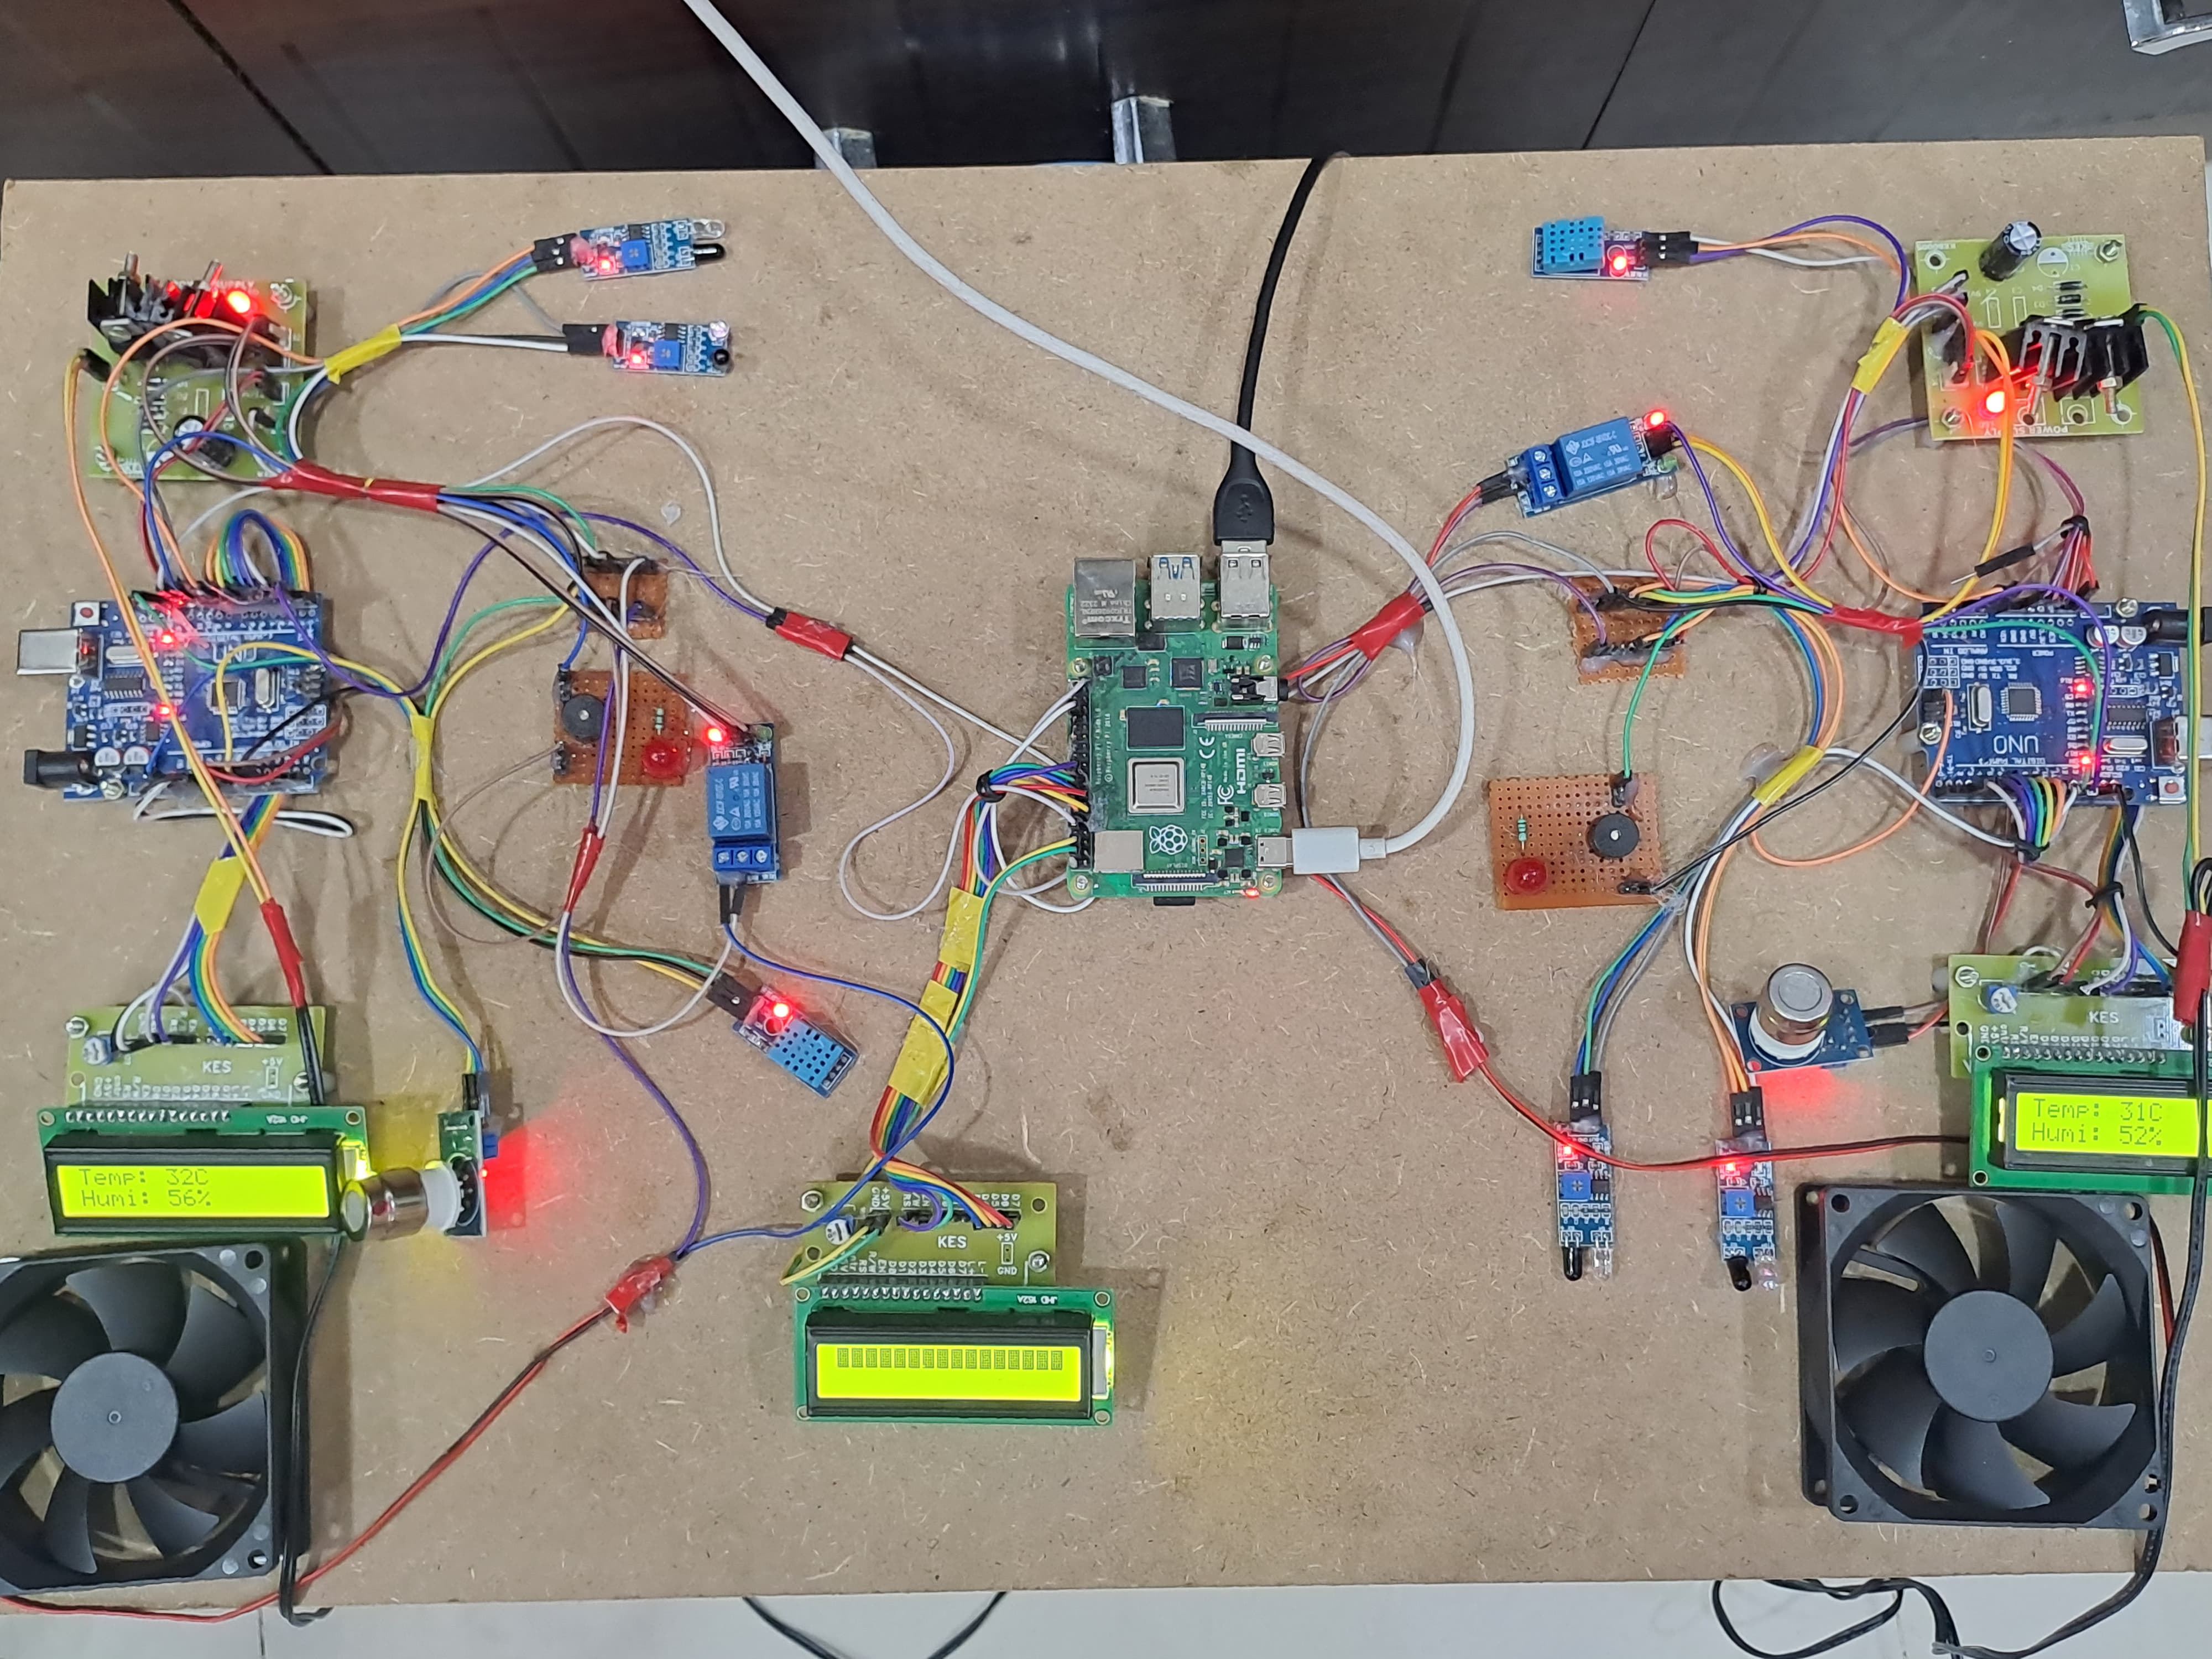
\includegraphics[width=\columnwidth]{figures/kit.jpg.jpeg} % Changed width
  \caption{Hardware Implementation of the Edge-Based IoT System.}
  \label{fig:hardware_photo}
\end{figure}

\subsection{Data Collection and System Operation}
Real-time sensor data was successfully collected and processed by the Edge and Fog layers. ThingSpeak visualizations (Figures~\ref{fig:thingspeak_cls1} and \ref{fig:thingspeak_cls2}) confirmed consistent data logging. During the monitored period, observed environmental parameters included:
\begin{itemize}
    \item Temperature: Fluctuating generally between 31.0°C and 32.0°C.
    \item Humidity: Varying between 36.0\% and 40.0\%.
    \item CO\textsubscript{2}: Concentrations typically observed between 11-13 ppm in the provided sample, but showing potential spikes correlating with occupancy or ventilation changes (as suggested by the description of graphs in the thesis).
    \item Occupancy: Variable rates observed, reflecting classroom usage patterns.
\end{itemize}
The system demonstrated its ability to process this data in real-time, calculate the KPIv and Room Quality Score, and provide actionable recommendations. Log outputs and LCD displays (Figure~\ref{fig:lcd_output}) confirmed the system's capability to compare classroom conditions and suggest the optimal room based on calculated scores (e.g., recommending Classroom 1 with a score of 61.35 over Classroom 2 with 114.74 in one instance).

\begin{figure}[t]
  \centering
  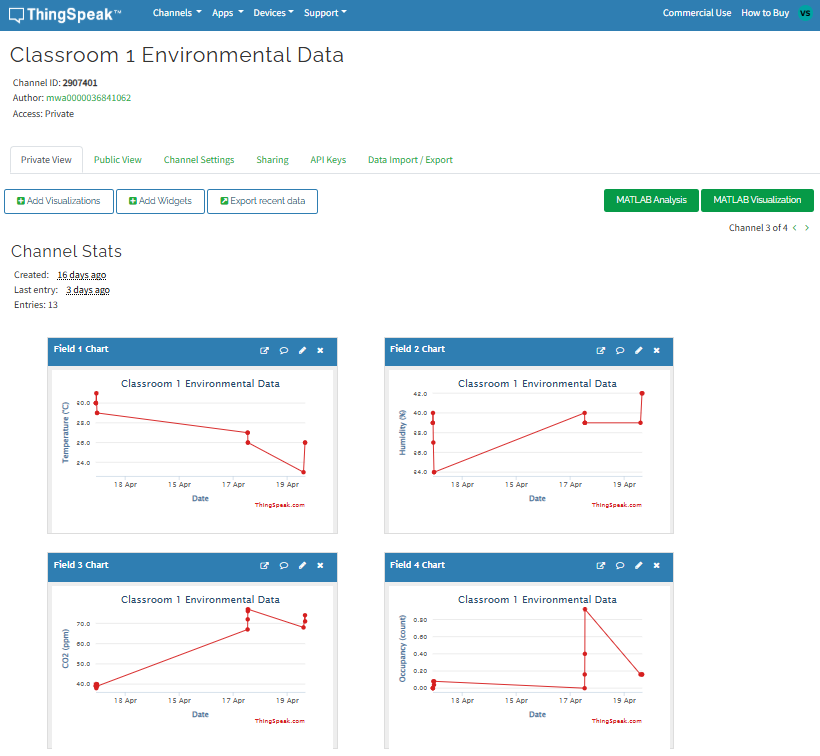
\includegraphics[width=\columnwidth]{figures/cls1.png} % Changed width
  \caption{ThingSpeak Data Visualization for Classroom 1.}
  \label{fig:thingspeak_cls1}
\end{figure}

\begin{figure}[t]
  \centering
  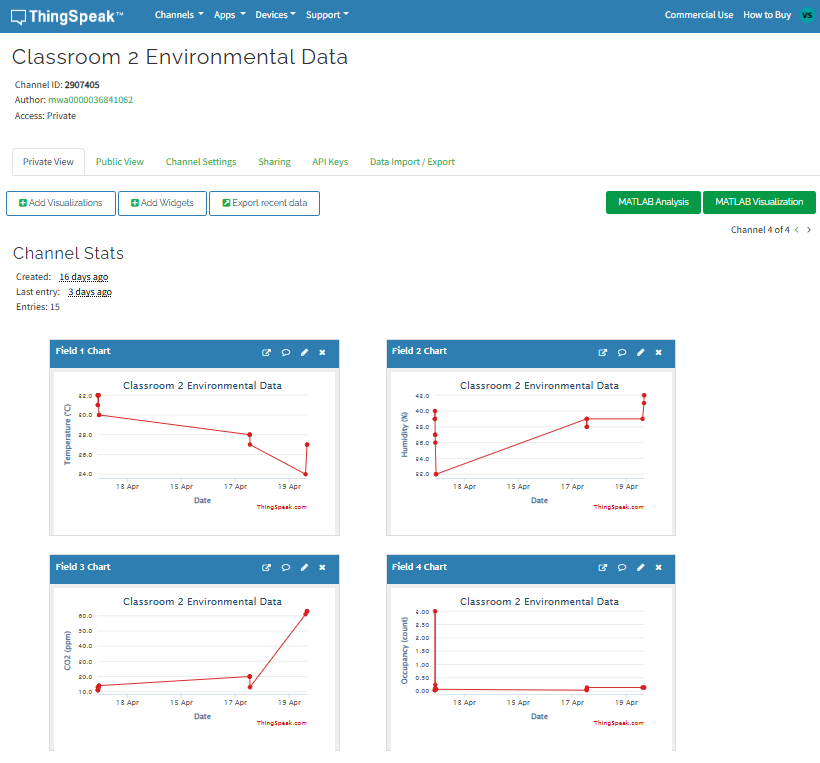
\includegraphics[width=\columnwidth]{figures/cls2.png} % Changed width
  \caption{ThingSpeak Data Visualization for Classroom 2.}
  \label{fig:thingspeak_cls2}
\end{figure}

\begin{figure}[t]
  \centering
  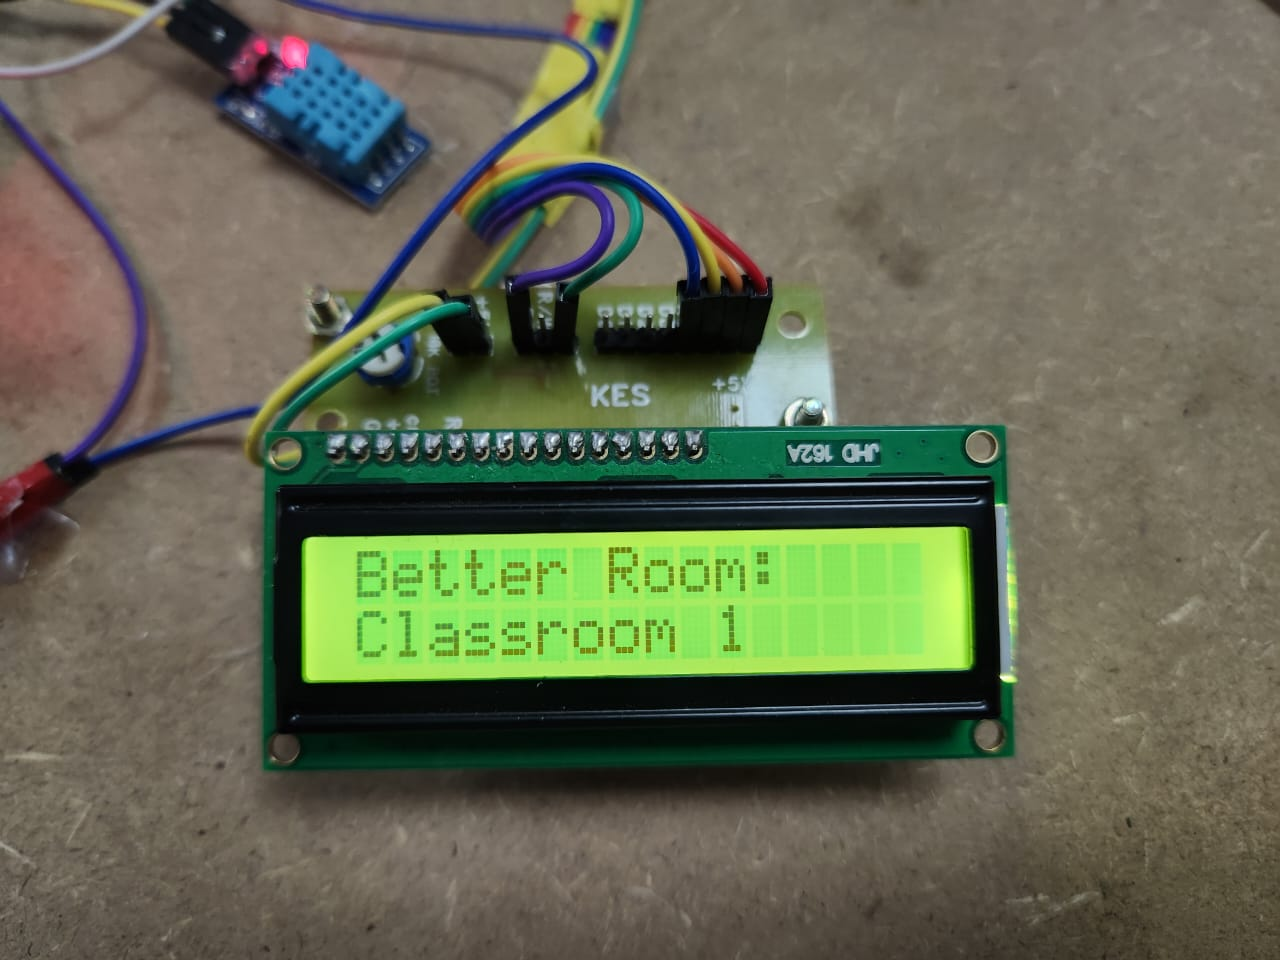
\includegraphics[width=0.8\columnwidth]{figures/lcd.jpeg} % Changed width
  \caption{LCD Output Display Indicating Recommendation of Optimal Classroom.}
  \label{fig:lcd_output}
\end{figure}

\subsection{LSTM Model Performance}
The LSTM model was trained offline on a harmonized dataset derived from multiple sources, preprocessed using forward-fill for missing values and Min-Max scaling, and structured into sequences of 10 timesteps. The training utilized the Adam optimizer and Mean Squared Error (MSE) loss, running for 5 epochs with early stopping and learning rate adjustment (as detailed in Section \ref{sec:methodology}). The pre-trained model, evaluated on the test set, achieved a final loss (MSE) of 0.0012 and a Mean Absolute Error (MAE) of 0.0143. This level of performance indicates the model's capability to predict environmental trends with reasonable accuracy. The trained model, deployed on the Fog layer (Raspberry Pi), successfully processed real-time sensor sequences to generate predictions. The system's ability to utilize these predictions alongside current data for calculating KPIv and Room Quality Score confirms the practical integration of the ML model into the control loop.

\subsection{Certificate Generation}
The automated certificate generation component successfully processed the collected environmental data stored via ThingSpeak. A sample generated certificate (Figure~\ref{fig:certificate_example}) demonstrated the system's ability to:
\begin{itemize}
    \item Aggregate data over a specified period (e.g., 6 readings shown).
    \item Calculate average, minimum, and maximum values for key parameters (Temp, Humidity, CO\textsubscript{2}, Occupancy).
    \item Compute the KPIv based on the collected data.
    \item Assign an overall environmental quality grade (e.g., A+ with a score of 95/100 achieved in the sample).
\end{itemize}
This validates the end-to-end functionality of the system, from data collection and analysis to formal quality reporting.

\begin{figure}[t]
  \centering
  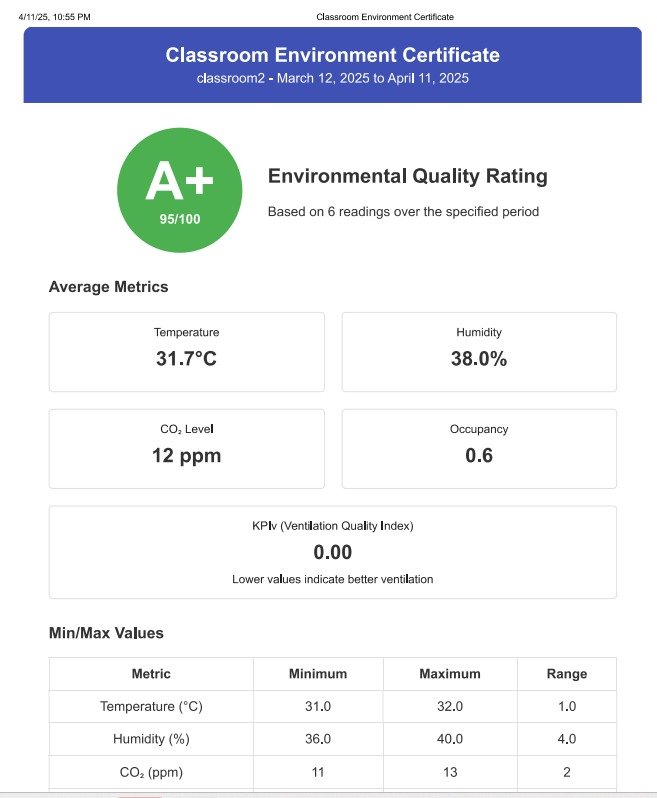
\includegraphics[width=\columnwidth]{figures/image (4).png} % Changed width
  \caption{Example Generated Classroom Environmental Quality Certificate.}
  \label{fig:certificate_example}
\end{figure}

Overall, the results demonstrate the feasibility and effectiveness of the proposed edge-driven system in monitoring classroom environments, utilizing LSTM predictions for intelligent assessment, and providing automated control and quality certification. 